\section{SSH to FutureSystems Resources}

Next, you need to upload the key to the portal. You must be logged into
the portal to do so.

\begin{description}
\item[Step 1:] Log into the portal

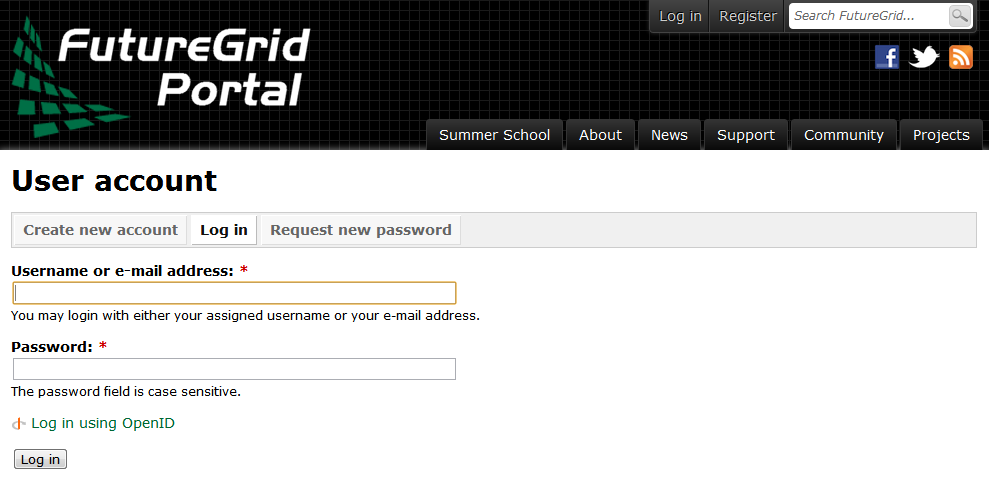
\includegraphics[width=0.5\textwidth]{/images/portalLogin_0.png}

\item[Step 2:] Click in the ``ssh key'' button. or go directly to
\url{https://portal.futuresystems.org/my/ssh-keys}

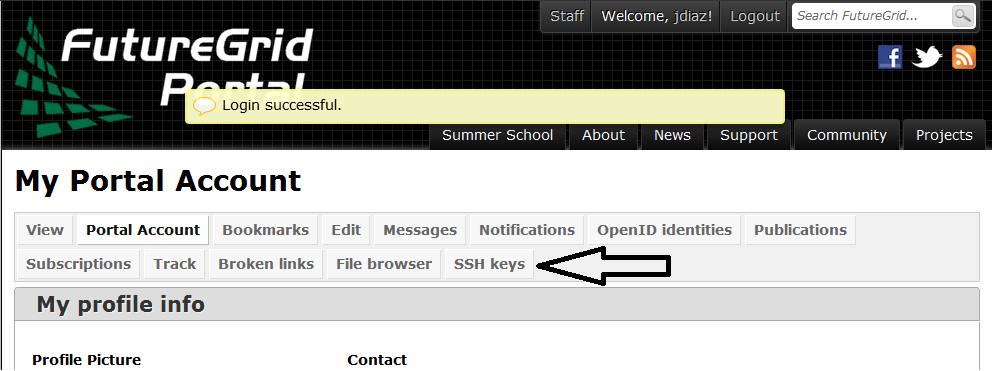
\includegraphics[width=0.5\textwidth]{/images/portalsshkey.png}

\item[Step 3:] Click in the ``add a public key'' link.

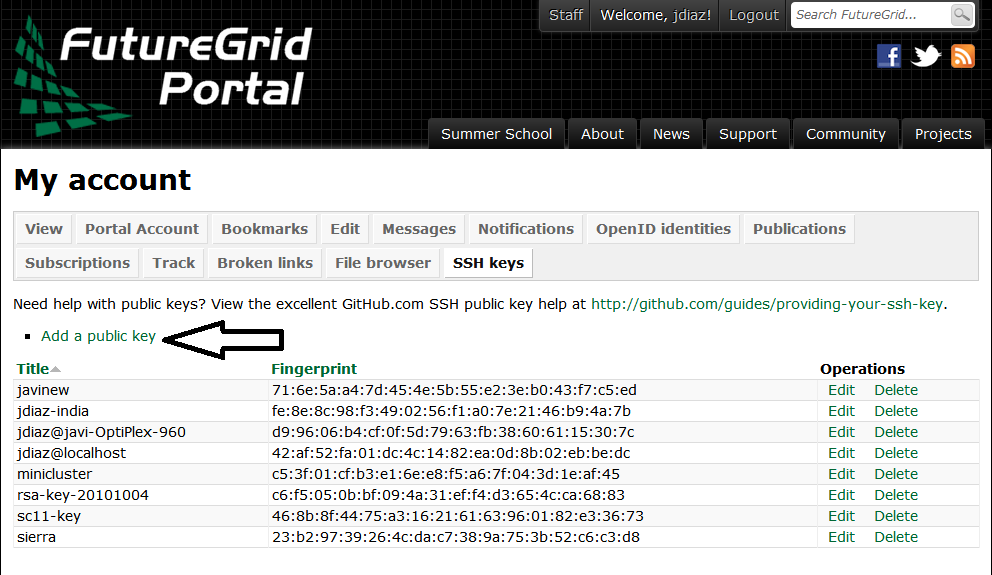
\includegraphics[width=0.5\textwidth]{/images/portalclikaddkey_0.png}

\item[Step 4:] Paste your ssh key into the box marked Key. Use a text
editor
to open the ``id\_rsa.pub''. Copy the entire contents of this file into
the ssh key field as part of your profile information. Many errors are
introduced by users in this step as they do not paste and copy
correctly.
\end{description}

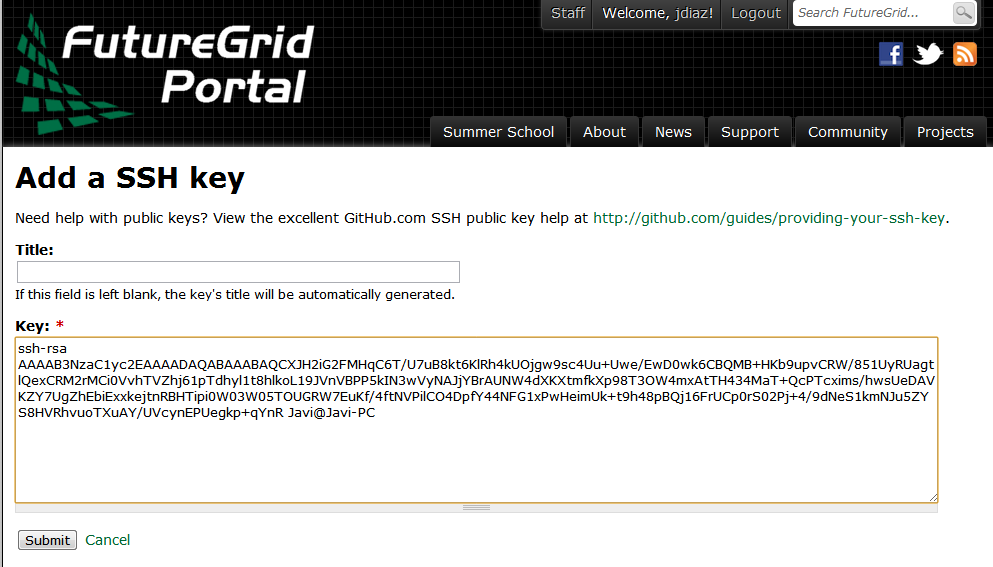
\includegraphics[width=0.5\textwidth]{/images/portalkeypaste_0.png}

Step 5: Click the submit button. \textbf{IMPORTANT}: Leave the
Title field blank.]
Make sure that when you paste your key, it does not contain newlines or
carriage returns that may have been introduced by incorrect pasting and
copying. If so, please remove them.


At this point, you have uploaded your key. However, you will still need
to wait till all accounts have been set up to use the key, or if you did
not have an account till it has been created by an administrator.
Please, check your email for further updates. You can also refresh this
page and see if the boxes in your account status information are all
green. Then you can continue.

\section{Testing your ssh key}\label{testing-your-ssh-key}

If you have had no FutureSystem account before, you need to wait for up
to two business days so we can verify your identity and create the
account. So please wait. Otherwise, testing your new key is almost
instantaneous on india. For other clusters like it can take around 30
minutes to update the ssh keys.

To log into india simply type the usual ssh command such as:

\begin{verbatim}
$ ssh portalname@india.futuresystems.org
\end{verbatim}

The first time you ssh into a machine you will see a message like this:

\begin{verbatim}
The authenticity of host 'india.futuresystems.org (192.165.148.5)' can't be established.
RSA key fingerprint is 11:96:de:b7:21:eb:64:92:ab:de:e0:79:f3:fb:86:dd.
Are you sure you want to continue connecting (yes/no)? yes 
\end{verbatim}

You have to type yes and press enter. Then you will be logging into
india. Other FutureSystem machines can be reached in the same fashion.
Just replace the name india, with the appropriate FutureSystems resource
name.
